\begin{center}
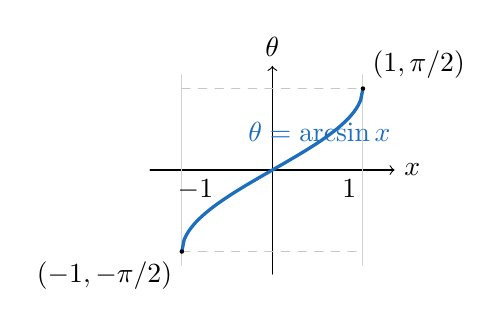
\begin{tikzpicture}[scale=1.15, line cap=round, line join=round]
  \definecolor{trigblue}{RGB}{30,110,190}
  \draw[->] (-1.35,0)--(1.35,0) node[right] {$x$};
  \draw[->] (0,-1.15)--(0,1.15) node[above] {$\theta$};
  \draw[gray!35] (-1,-1.05)--(-1,1.05);
  \draw[gray!35] (1,-1.05)--(1,1.05);
  \draw[gray!45,dashed] (-1,-0.9)--(1,-0.9);
  \draw[gray!45,dashed] (-1,0.9)--(1,0.9);
  \draw[very thick,trigblue,domain=-1:1,samples=80]
    plot ({\x},{0.9*asin(\x)/90});
  \fill (-1,-0.9) circle (0.025) node[below left] {$(-1,-\pi/2)$};
  \fill (1,0.9) circle (0.025) node[above right] {$(1,\pi/2)$};
  \node[trigblue] at (0.52,0.42) {$\theta=\arcsin x$};
  \node[below] at (0.85,0) {$1$};
  \node[below] at (-0.85,0) {$-1$};
\end{tikzpicture}
\end{center}


\begin{definitionbox}{Definition}
\begin{definition}[Inverse sine]
\label{def:inverse-sine}
The \emph{inverse sine} function is the inverse of sine after sine is
restricted to the interval
\[
  \left[-\frac{\pi}{2},\frac{\pi}{2}\right].
\]
It is denoted by $\arcsin$ or $\sin^{-1}$ and has domain $[-1,1]$ and range
$[-\pi/2,\pi/2]$.
\[
  \arcsin x=\theta
  \quad\Longleftrightarrow\quad
  \sin\theta=x
  \quad\text{and}\quad
  -\frac{\pi}{2}\leq\theta\leq\frac{\pi}{2}.
\]
\end{definition}
\end{definitionbox}
\begin{remark*}[Domain and range]
The full sine function has domain all real-valued angle measures and range
$[-1,1]$. The inverse sine function reverses the restricted sine function, so
its domain is $[-1,1]$ and its range is the principal interval
$[-\pi/2,\pi/2]$.
\end{remark*}
\begin{dependencies}
\begin{itemize}
  \item \hyperref[def:unit-circle-sine]{Unit-circle sine}
  \item \hyperref[def:radian-measure]{Radian measure}
\end{itemize}
\end{dependencies}

\begin{theorembox}{Theorem}
\begin{theorem}[Principal inverse sine identities]
\label{thm:inverse-sine-identities}
For every $x\in[-1,1]$,
\[
  \sin(\arcsin x)=x.
\]
For every $\theta\in[-\pi/2,\pi/2]$,
\[
  \arcsin(\sin\theta)=\theta.
\]
\end{theorem}
\end{theorembox}
\begin{remark*}[Standard quantified statement]
\[
  \forall x\in[-1,1],\quad \sin(\arcsin x)=x,
  \qquad
  \forall \theta\in[-\pi/2,\pi/2],\quad \arcsin(\sin\theta)=\theta.
\]
\end{remark*}
\begin{dependencies}
\begin{itemize}
  \item \hyperref[def:inverse-sine]{Inverse sine}
\end{itemize}
\end{dependencies}
